\chapter{Introducción}\label{ch:introduccion}
La microscopia óptica representa una fracción muy importante de los desarrollos experimentales en campos de gran importancia en la física desde su invención, y se ha convertido en un instrumento vital para un científico que quiera generar aportes significativos en su campo de estudio. Teniendo en cuenta su importancia, se esperaría que el acceso a microscopios de alta potencia y desempeño estuviera a la mano de cualquiera que estuviera dispuesto a usarlo; sin embargo, existe el problema del costo elevado para el desarrollo de microscopia de alto nivel, y se presenta el reto de desarrollar microscopios de un rendimiento alto que pueda ser accesible a cualquiera en términos económicos. Se han hecho muchos esfuerzos en campos como la biología, la química, la física y la medicina con el fin de lograr el cometido de generar la visualización de alta calidad aplicando técnicas no convencionales \cite{Zhang2016} o haciendo uso de dispositivos de tamaño reducido \cite{Coskun2010, Greenbaum2012}. Es importante remarcar que un microscopio de buena calidad no sólo se compone de una buena etapa de detección óptica, sino que en el caos de la presencia de campos de visión muy grandes se debe contar con un stage mecánico que le permita desplazarse a través de toda el área de interés, y esto se vuelve mucho más crítico cuando la resolución es alta y, por lo tanto, se debe ser muy cuidadoso en la velocidad del movimiento de esta  etapa \cite{Abramowitz2015, Kim2008}.

Con este fin, este proyecto busca generar un stage con capacidad de muestrear la totalidad del volumen de una muestra y con bajo costo de fabricación que pueda, en conjunto con una etapa de detección óptica que se ajuste a las dimensiones del mismo, cumplir la función de un microscopio de alto desempeño para la obtención de resultados ópticos. Esto se logró a partir del desarrollo de una etapa de movimiento mecánico en tres dimensiones, que funciona gracias a la presencia de un motor encargado de desplazar el dispositivo en cada dirección, y una serie de desarrollos de código que controlan el movimiento del stage y permiten generar un plano de enfoque para tener en cuenta lo posibles desniveles de la muestra posicionada bajo la etapa de detección. El documento presenta detalladamente los desarrollos anteriormente descritos, presenta un contexto teórico que permite al lector encontrar las bases del desarrollo, presenta resultados en forma de imágenes y métricas de desempeño del movimiento y finaliza con una discusión acerca de cómo esto podría ser implementado y presenta una serie de conclusiones de todo el trabajo realizado.

\section{Marco teórico}
Dentro de las piezas de mayor importancia de un microscopio óptico se encuentra el stage. En la gran mayoría de los casos estos no son motorizados, restringiendo la reproducibilidad de estudios que requieran estudiar el área total de la muestra. Por otro lado la manipulación de un stage, en caso de no realizarse con el debido cuidado puede dar lugar a la descalibración de partes sensibles del microscopio. La velocidad con la que un ser humano puede manipular el stage puede ser relativamente alta, sin embargo está lejos de ser constante, razón por la cual cuando se quieren hacer estudios de larga exposición o que requieran el movimiento constante de la muestra es necesario un stage automatizado.
\begin{figure}[h]
	\centering
	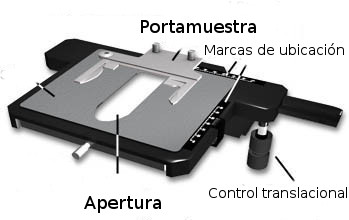
\includegraphics[width=0.5\linewidth]{figures/stage1.jpg}
	\caption{Stage mecánico convencional. Modificado de \cite{Abramowitz2015}.}
\end{figure}

Si bien la automatización permite resolver varios problemas, también se debe tener en cuenta la susceptibilidad a otros. En el caso de un stage en $x$ y $y$ automatizado, al barrer gran cantidad de área se vuelve necesario una preparación de la muestra exhaustiva para limitar cambios significativos en el grosor de la misma que afecten el enfoque sobre el microscopio. Por esta razón se plantea la construcción del stage con una motorización adicional en la dirección $z$.

Existen tres tipos de motores de fácil acceso en el mercado local. Cada uno de ellos con ventajas y desventajas respecto a los demás.
\begin{itemize}
	\item \textbf{Motores de escobillas:} Son los más comunes en el mercado, pues se usan con frecuencia en juguetes, electrodomésticos y accesorios para computadores. Entre sus ventajas se encuentra la velocidad de rotación de los mismos y el torque que generan. Son operados con voltajes análogos. Su desventaja consiste en el control preciso de la posición.  
	\item \textbf{Servo motores:} Los servomotores son usados en aplicaciones donde no se requieren rotaciones completas, pero sí precisión en la ubicación del mismo. Para su manipulación es necesario el uso de frecuencia modulada, es decir realizar pulsaciones sobre salidas digitales. Su gran desventaja es la incapacidad de realizar rotaciones mayores a 180 $^\circ$ y el poco torque que ejercen.
	\item \textbf{Motores de paso:} Este tipo de motores no presenta escobillas, usando un imán y una serie de bobinas separadas entre sí, es posible determinar la orientación del mismo, logrando que este se quede en esa posición hasta que la bobina vecina sea activada. Son ideales para aplicaciones que requieran control de la posición con torques moderados, sin embargo su velocidad de rotación está restringida a la frecuencia de pulsación de cada bobina.
	
	\begin{figure}[h]
		\centering
		\begin{tabular}{ccc}
			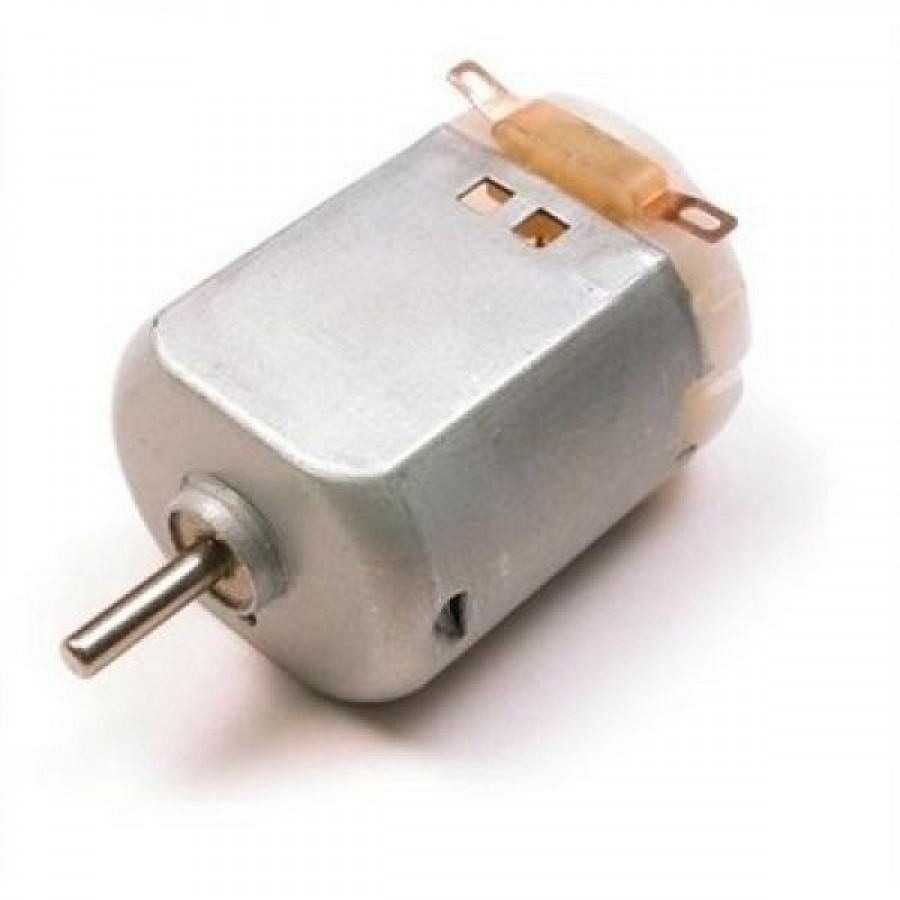
\includegraphics[width = 0.3\linewidth]{figures/brushed.jpg} &
			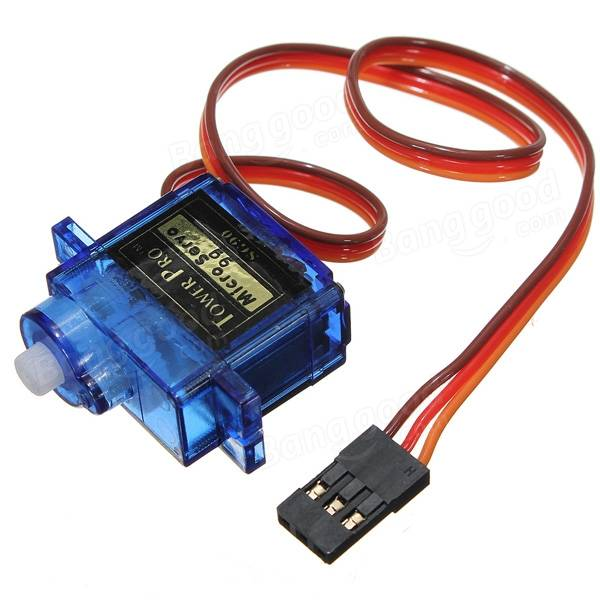
\includegraphics[width = 0.3\linewidth]{figures/stepper.JPG} & 
			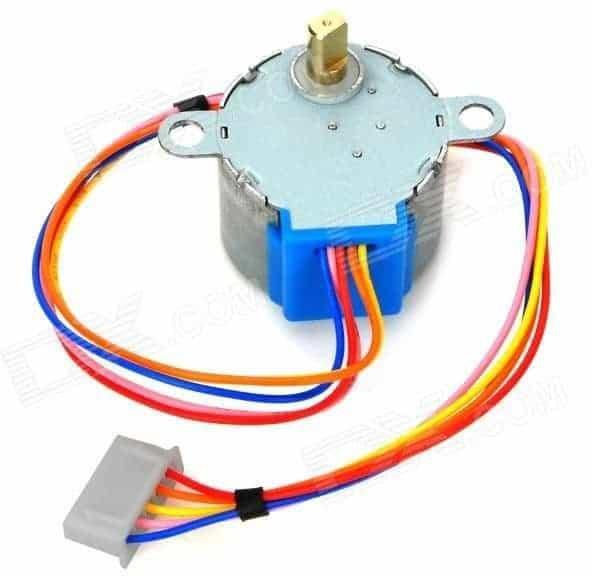
\includegraphics[width = 0.3\linewidth]{figures/paso.jpg}
		\end{tabular}
		\caption{Motores adquiridos para la realización del proyecto. De izquierda a derecha: motor de escobillas, servo y de paso.}
	\end{figure}
\end{itemize}

Finalmente y con el objetivo de realizar el control de los distintos motores, se debe usar un microcontrolador, el cual permita establecer comunicación con el computador para la recepción de instrucciones, y la habilidad de generar los pulsos necesarios para la activación de determinado motor. Entre los requerimientos que este debe tener se encuentran los puertos UART, los cuales permitirán llevar a cabo la comunicación por puerto serial con el computador.